\chapter{粒子力学、四维动量与静止能量}

\section{我们将反复使用的近似}

相对论性粒子的力学必须用新的语言回答熟悉的问题。粒子如何运动？它的动量和能量是什么？为什么这些量能组合成一个四维矢量，以及\(E=mc^2\)如何从力学的通常机制中产生？在讨论这些问题之前，我们需要一个初等的近似，它将在整个计算中反复出现。

对任意指数\(p\)，二项级数为
\begin{equation}
\begin{aligned}
(1+\epsilon)^p
&=1+p\epsilon\\
&\quad+\frac{p(p-1)}{2!}\epsilon^2\\
&\quad+\frac{p(p-1)(p-2)}{3!}\epsilon^3
+\cdots .
\end{aligned}
\label{eq:sr3-binomial}
\end{equation}
该指数可以是正数、负数、分数，甚至复数。对足够小的\(\epsilon\)，级数收敛很快，且每一项都比前一项小。于是我们可以在所需精度要求的任意阶处截断。零阶项通常是最大的，但在下面的应用中它常常是常数，因而在动力学上无趣。运动出现在一阶修正中。

\begin{figure}[htbp]
\centering
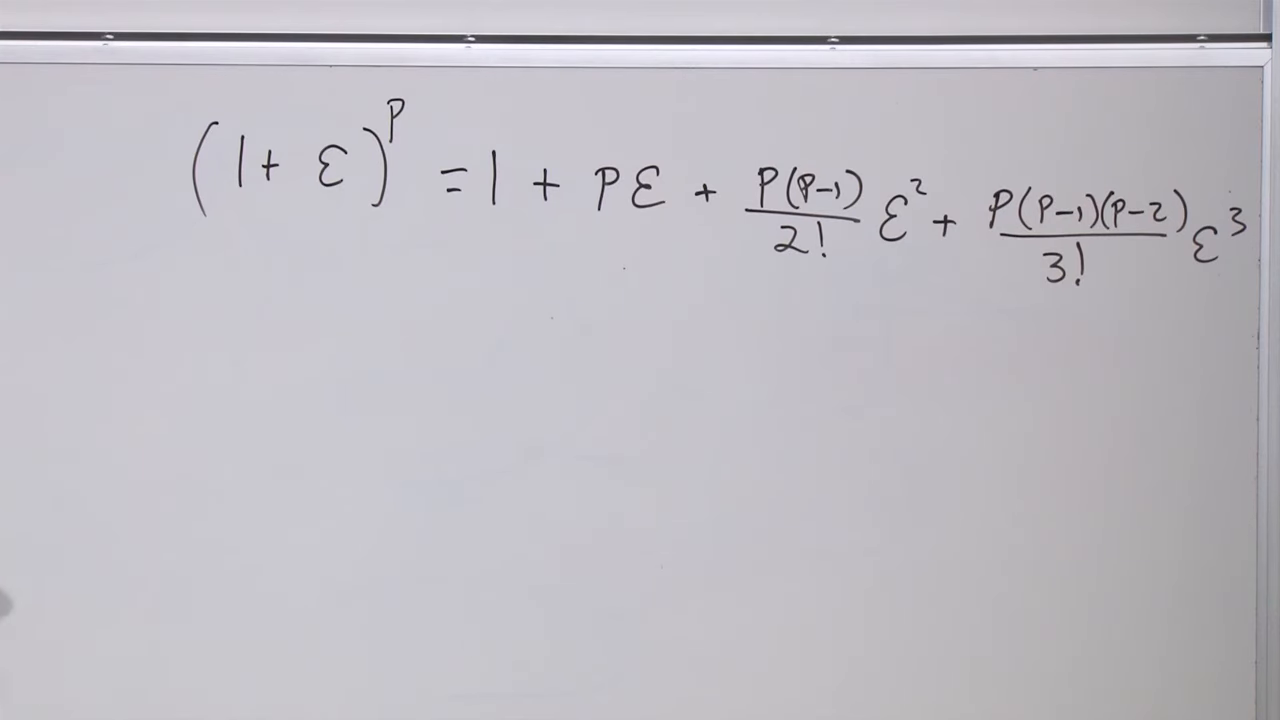
\includegraphics[width=0.90\textwidth]{lecture_03_figure_01.png}
\caption{二项级数展开到三阶，用于从相对论公式恢复非相对论力学。}
\lectureframe{00:04:24}
\end{figure}

我们通常取\(c=1\)，因此速度\(v\)意味着光速的\(v/c\)倍。取\(\epsilon=-v^2\)。当\(p=\tfrac12\)时，
\begin{equation}
\sqrt{1-v^2}
=
1-\frac{v^2}{2}-\frac{v^4}{8}-\cdots
\approx
1-\frac{v^2}{2},
\qquad |v|\ll 1.
\label{eq:sr3-sqrt-expansion}
\end{equation}
当\(p=-\tfrac12\)时，两个负号相消：
\begin{equation}
\frac{1}{\sqrt{1-v^2}}
=
1+\frac{v^2}{2}+\frac{3v^4}{8}+\cdots
\approx
1+\frac{v^2}{2}.
\label{eq:sr3-gamma-expansion}
\end{equation}
经典力学中的许多\(1/2\)因子，事后可以辨认出是这些相对论展开式中的一阶修正。当\(v\)趋近于1时，该近似失效；此时任何有限截断都无法捕捉精确表达式的奇异行为。

\begin{figure}[htbp]
\centering
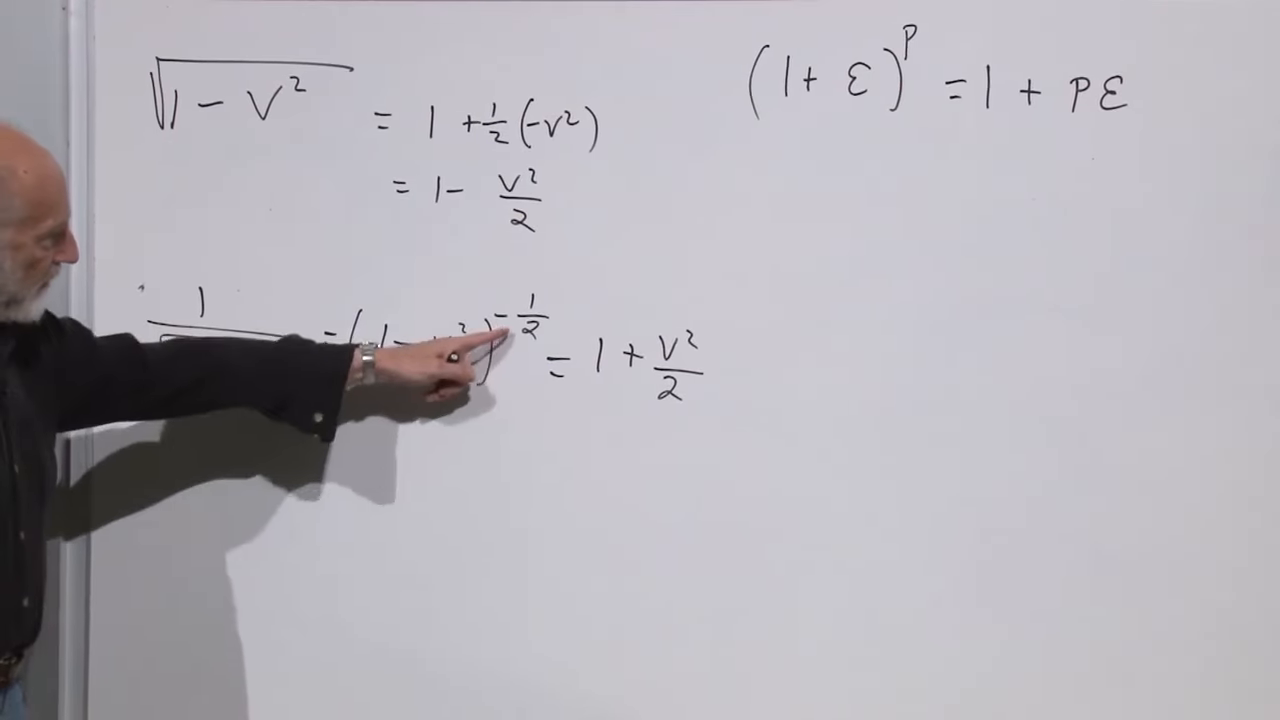
\includegraphics[width=0.90\textwidth]{lecture_03_figure_02.png}
\caption{两个低速公式都可见：\(\sqrt{1-v^2}\approx1-v^2/2\)和\((1-v^2)^{-1/2}\approx1+v^2/2\)。}
\lectureframe{00:07:39}
\end{figure}

\section{什么算作粒子？}

力学中的粒子不必是基本粒子。它可以是电子、太阳、一盒巧克力或一个甜甜圈。重要的是该物体足够紧密地保持在一起，使其整体运动可由质心描述。甜甜圈是一个有用的提醒：质心不必位于物质本身之内。

在牛顿力学中，质心变量满足
\begin{equation}
\vec p=m\vec v,
\qquad
K=\frac12mv^2,
\qquad
\vec F=m\vec a.
\label{eq:sr3-newtonian-particle}
\end{equation}
这些公式不关心物体是基本的还是复合的。复合物体还包含内能。例如，一个运动的甜甜圈具有质心动能加上化学能、热能和束缚能：
\begin{equation}
E_{\text{Newtonian}}
=
E_{\text{internal}}+\frac12mv^2.
\label{eq:sr3-newtonian-internal}
\end{equation}
内能项与整体质心速度无关。相对论将保留这一区分，但会揭示内能对整体物体的不变质量有贡献。

所需的工具与经典力学中使用的相同：轨迹、稳定作用量原理、拉格朗日量、正则动量、哈密顿量，以及连续对称性与守恒定律之间的关系。

\section{世界线与因果分离}

将系统的位置画在水平方向，时间画在竖直方向。它的历史便是时空中的一条曲线。对一个粒子而言，这条曲线就是它的\emph{世界线}。这一概念在牛顿力学中已经存在，但在相对论中它变得基础，因为洛伦兹变换混合了空间与时间。

考虑由下式分隔的两个事件
\begin{equation}
\Delta x^\mu=(\Delta t,\Delta\vec x),
\qquad
\Delta\vec x^{\,2}
=
(\Delta x)^2+(\Delta y)^2+(\Delta z)^2.
\end{equation}
在单位\(c=1\)下，它们的不变间隔为
\begin{equation}
(\Delta\tau)^2
=
(\Delta t)^2-\Delta\vec x^{\,2}.
\label{eq:sr3-interval}
\end{equation}

\subsection{类时间隔}

若\((\Delta t)^2>\Delta\vec x^{\,2}\)，则\((\Delta\tau)^2>0\)，该间隔为类时的。存在一个洛伦兹参考系，其中这两个事件发生在同一空间点。在该参考系中，连接它们的线是竖直的，一个时钟可以从一个事件旅行到另一个事件。它经过的读数是固有时\(\Delta\tau\)。

\begin{figure}[htbp]
\centering
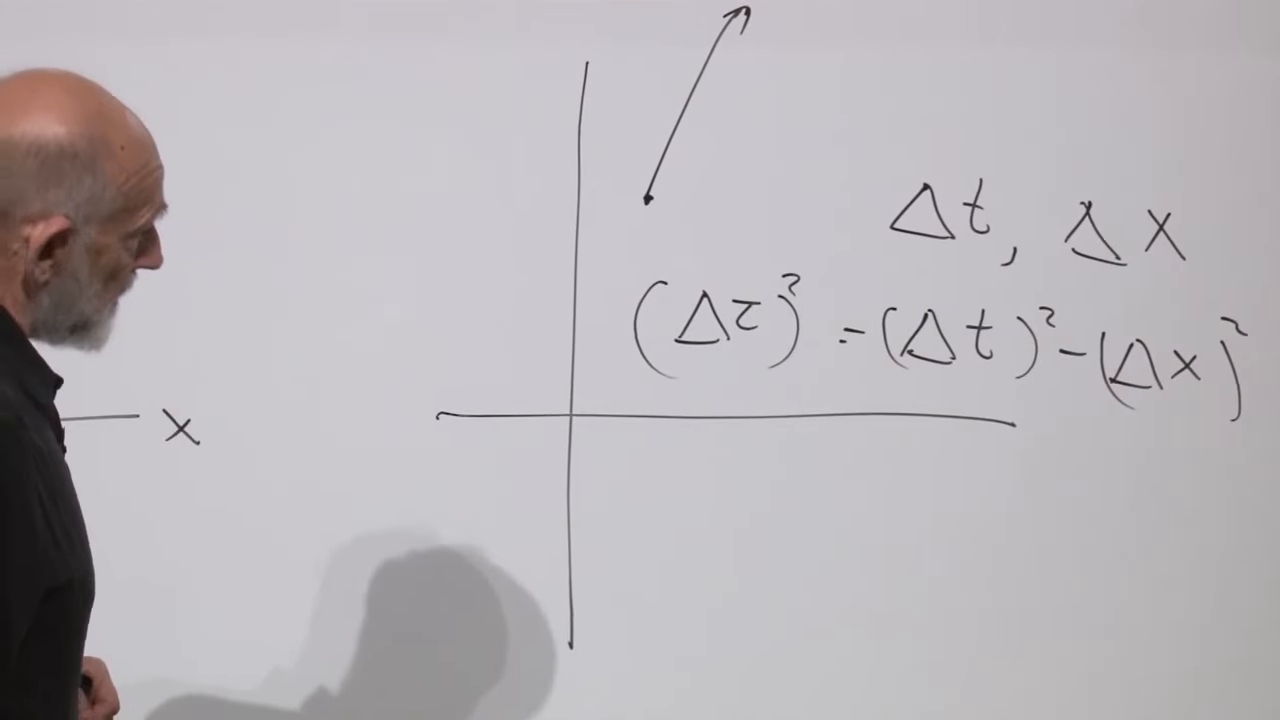
\includegraphics[width=0.90\textwidth]{lecture_03_figure_03.png}
\caption{类时间隔的时间分离大于空间分离；存在一个静止参考系，其中两个事件共享同一位置。}
\lectureframe{00:14:42}
\end{figure}

\subsection{类空间隔}

若\(\Delta\vec x^{\,2}>(\Delta t)^2\)，该间隔为类空的。没有任何惯性参考系能使两个事件处于同一空间点，但存在一个参考系使它们同时发生。其他参考系可以颠倒它们的时间顺序。因此，对于类空事件对，\emph{事件\(A\)先发生}和\emph{事件\(B\)先发生}都不是不变陈述。这就是几何形式的同时性相对性。

\begin{figure}[htbp]
\centering
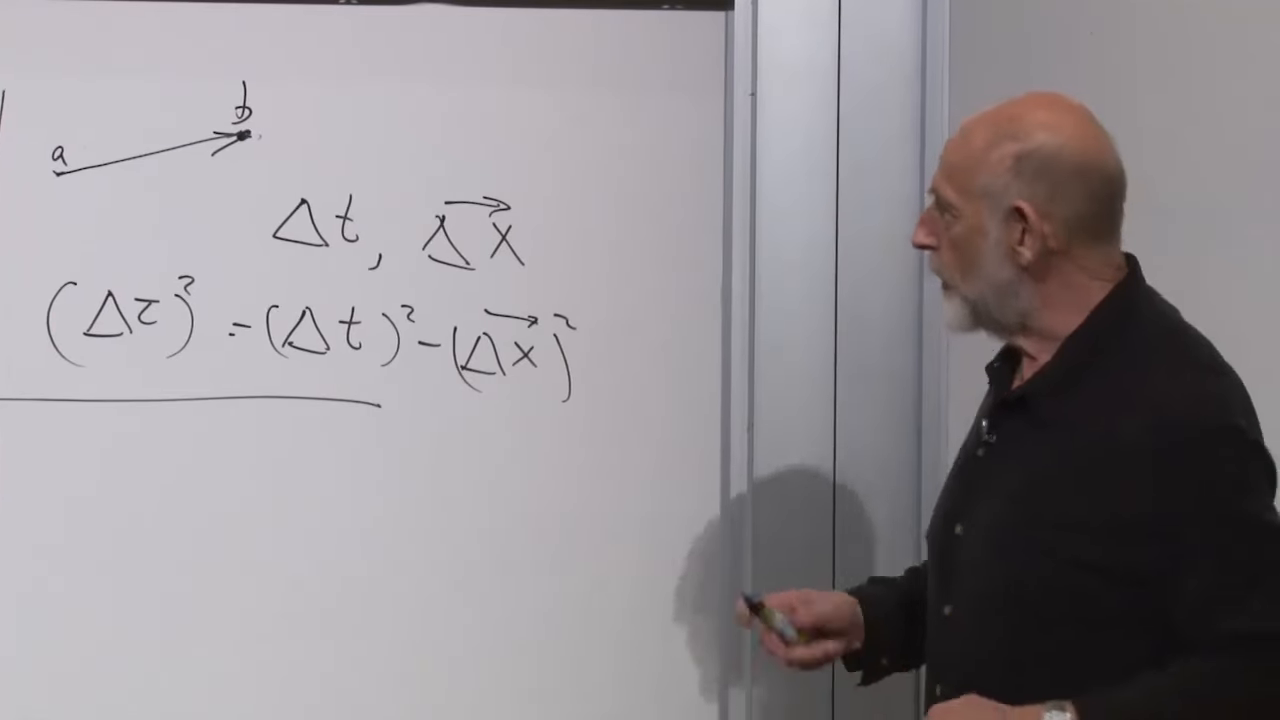
\includegraphics[width=0.90\textwidth]{lecture_03_figure_04.png}
\caption{对于类空间隔，惯性参考系的改变可以使两个事件同时发生或颠倒它们的时间顺序。}
\lectureframe{00:17:01}
\end{figure}

有质量粒子具有类时世界线：每一段足够短的线段都满足 \(d\tau^2>0\)。将 \(0.9c\) 的速度逐次合成，可以使粒子越来越接近 \(c\)，但永远不会超过它。这种趋近类似于芝诺悖论。这一因果限制不仅适用于物质客体，也适用于信号和信息，因为信息必须由物理系统携带。超光速信号会使不同参考系对其历史中哪一端是因、哪一端是果产生分歧。

\section{四维速度}

聚焦于一段短的类时线段。在常规单位下，
\begin{equation}
d\tau
=
\sqrt{dt^2-\frac{d\vec x^{\,2}}{c^2}}.
\label{eq:sr3-proper-time-dimensional}
\end{equation}
\(c^2\) 这个因子是由量纲强制得出的：\(dt^2\) 具有时间的平方的量纲，而 \(d\vec x^{\,2}\) 具有长度的平方的量纲。

\begin{classroomqa}
\audiencequestion{当间隔用普通单位写出时，光速必须插入在哪里？}
\lecturerresponse{空间项必须除以 \(c^2\)，得到 \(d\tau^2=dt^2-d\vec x^{\,2}/c^2\)。我们通常会回到 \(c=1\)，但量纲一致性总能恢复缺失的因子。\lecturetimestamp{00:21:23}}
\end{classroomqa}

\begin{figure}[htbp]
\centering
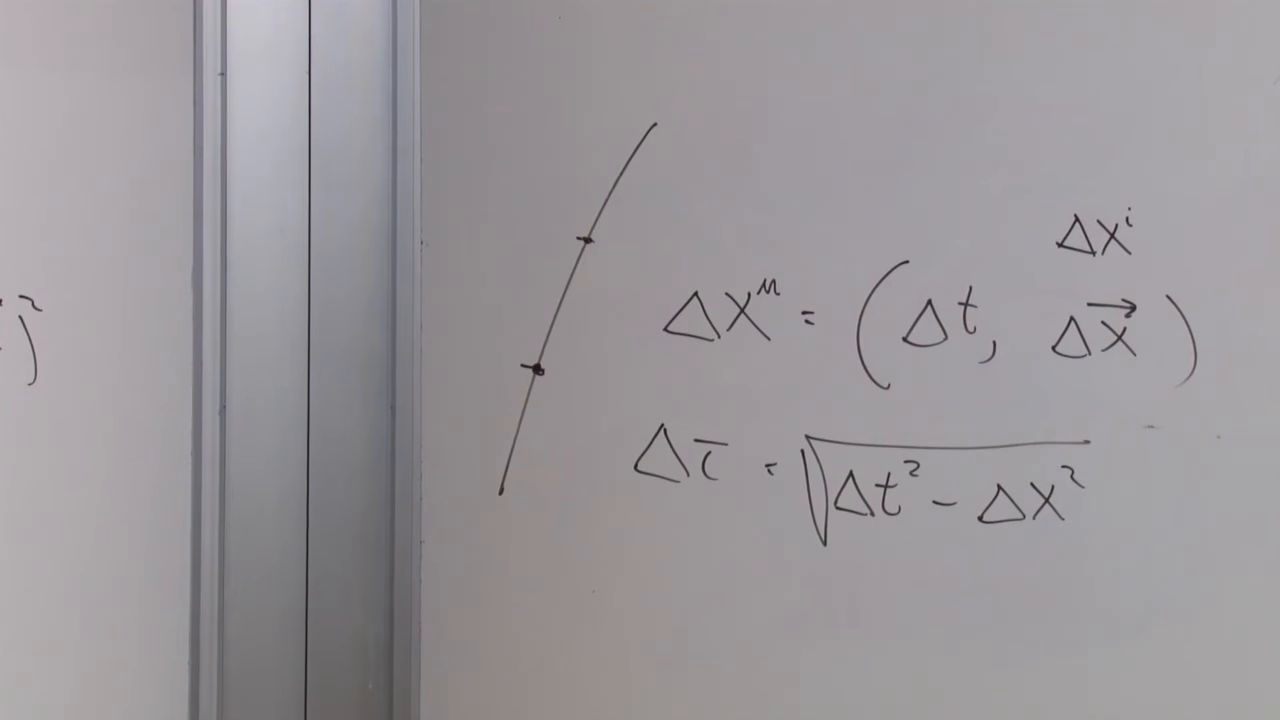
\includegraphics[width=0.90\textwidth]{lecture_03_figure_05.png}
\caption{世界线位移 \(\Delta x^\mu=(\Delta t,\Delta\vec x)\) 以及与之相关的固有时增量。}
\lectureframe{00:21:03}
\end{figure}

普通速度有三个空间分量，
\begin{equation}
v^i=\frac{dx^i}{dt},
\qquad i=1,2,3.
\end{equation}
相对论速度则是通过将完整的时空位移除以不变的固有时得到的：
\begin{equation}
u^\mu
=
\frac{dx^\mu}{d\tau},
\qquad
\mu=0,1,2,3.
\label{eq:sr3-four-velocity-definition}
\end{equation}
希腊指标遍历时空；拉丁指标遍历空间。在 \(c=1\) 单位下，位置的第零分量为 \(x^0=t\)，因此
\begin{equation}
u^0=\frac{dt}{d\tau}.
\end{equation}

\begin{figure}[htbp]
\centering
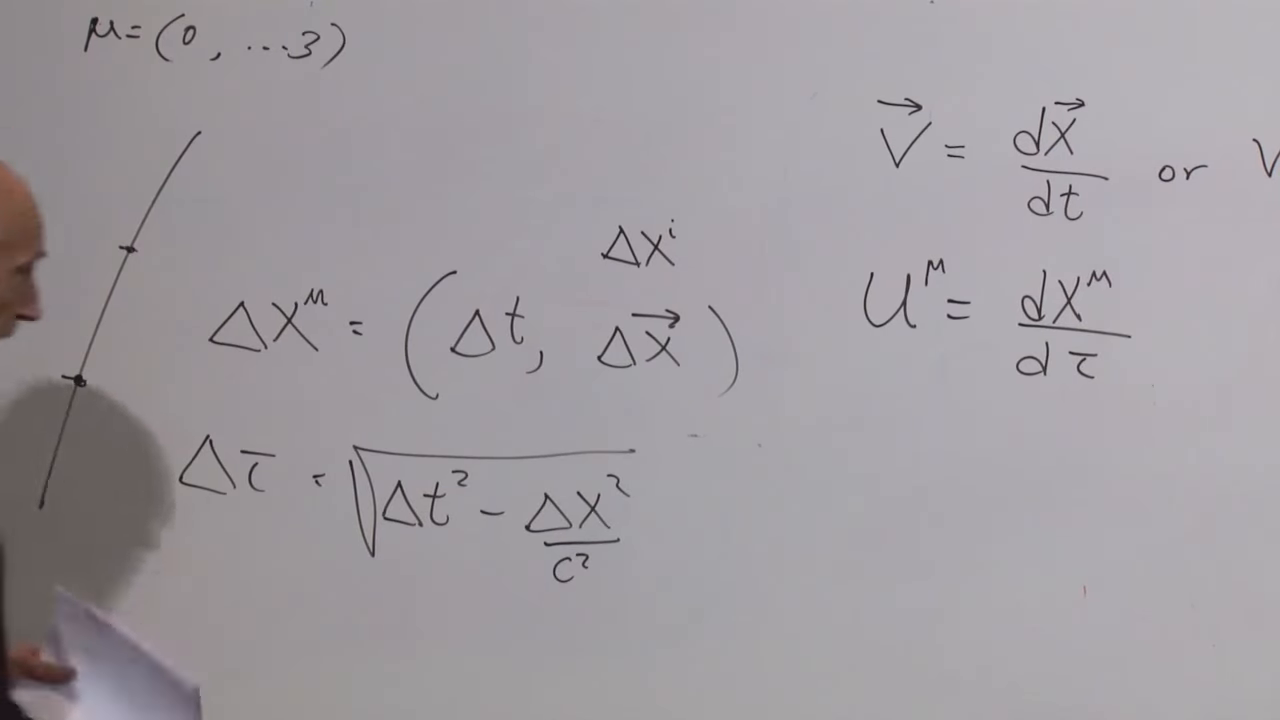
\includegraphics[width=0.90\textwidth]{lecture_03_figure_06.png}
\caption{普通速度将空间位移除以坐标时间，而四维速度则将全部四个分量除以固有时。}
\lectureframe{00:24:05}
\end{figure}

为了将 \(u^\mu\) 与 \(\vec v\) 联系起来，从间隔中提取因子 \(dt^2\)：
\begin{align}
d\tau^2
&=dt^2-d\vec x^{\,2}\\
&=dt^2\left(1-\frac{d\vec x^{\,2}}{dt^2}\right)
=dt^2(1-v^2).
\end{align}
对于指向未来的世界线取正根，
\begin{equation}
\frac{d\tau}{dt}=\sqrt{1-v^2},
\qquad
\frac{dt}{d\tau}=\frac{1}{\sqrt{1-v^2}}
\equiv\gamma.
\label{eq:sr3-time-component}
\end{equation}
对于空间分量，
\begin{equation}
v^i
=
\frac{dx^i}{dt}
=
\frac{dx^i}{d\tau}\frac{d\tau}{dt}
=u^i\sqrt{1-v^2}.
\end{equation}
因此
\begin{equation}
\boxed{
u^\mu
=
\gamma(1,\vec v)
},
\qquad
u^0=\gamma,
\qquad
u^i=\gamma v^i.
\label{eq:sr3-four-velocity-components}
\end{equation}
在低速下 \(u^0\to1\) 且 \(u^i\to v^i\)。接近光速时，即使 \(|\vec v|<1\)，\(u^0\) 和空间四维速度的大小都会变得很大。

\begin{figure}[htbp]
\centering
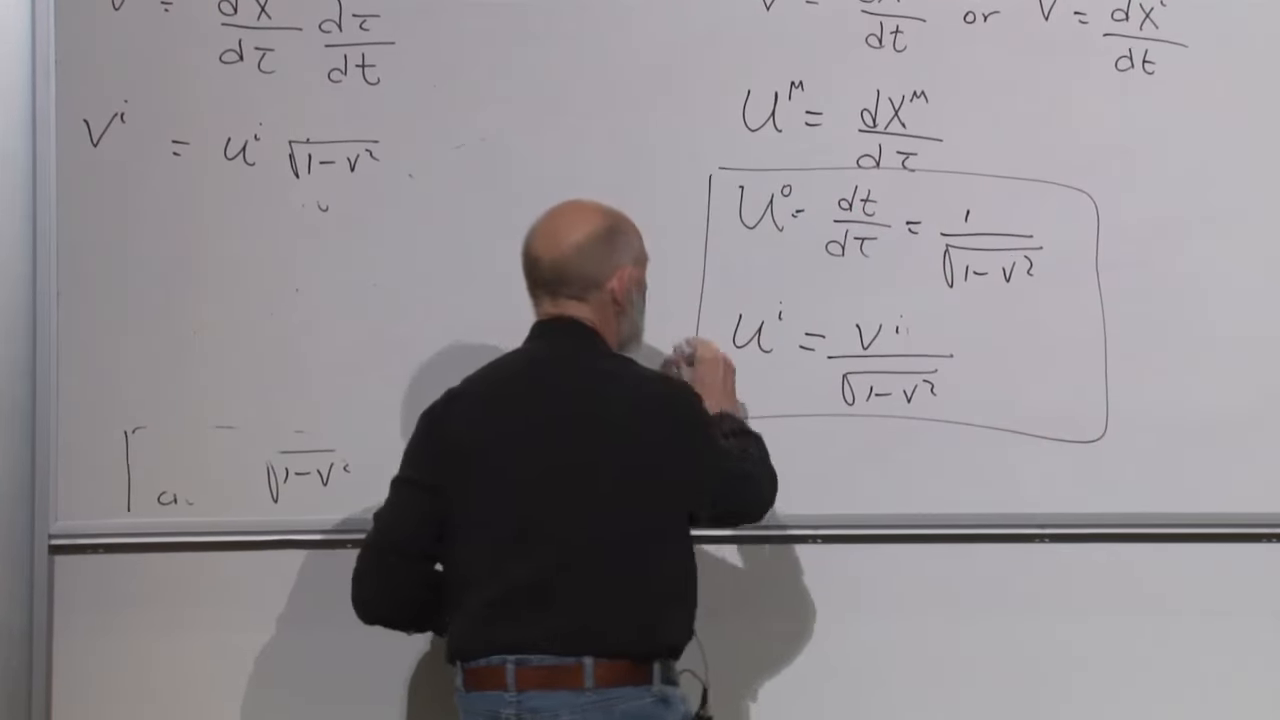
\includegraphics[width=0.90\textwidth]{lecture_03_figure_07.png}
\caption{普通速度与 \(u^\mu\) 的全部四个分量之间已确定的关系。}
\lectureframe{00:30:40}
\end{figure}

\subsection{为什么只有三个分量是独立的}

四维速度有四个分量，但只有三个独立的自由度。将间隔恒等式除以 \(d\tau^2\) 得到
\begin{equation}
1
=
\left(\frac{dt}{d\tau}\right)^2
-\left(\frac{d\vec x}{d\tau}\right)^2,
\end{equation}
或
\begin{equation}
\boxed{
(u^0)^2-\vec u^{\,2}=1
}.
\label{eq:sr3-four-velocity-normalization}
\end{equation}
这一个归一化条件消去了一个独立分量。

\begin{figure}[htbp]
\centering
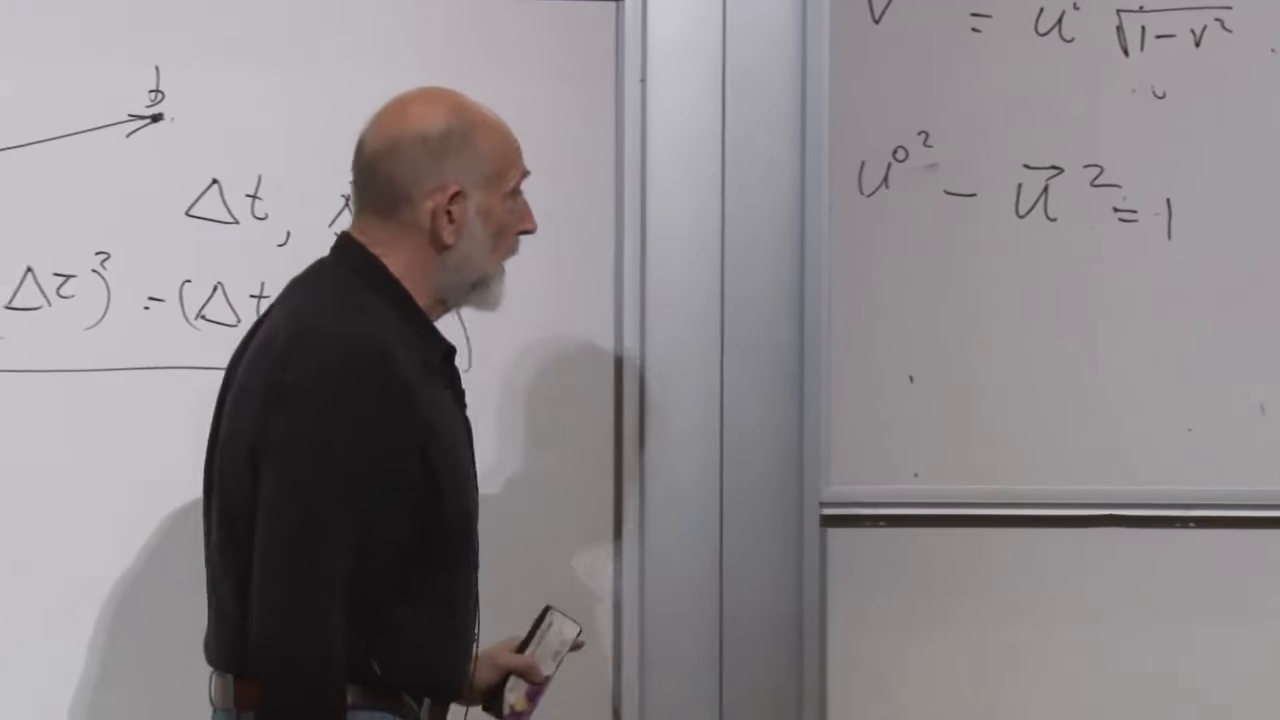
\includegraphics[width=0.90\textwidth]{lecture_03_figure_08.png}
\caption{不变间隔立即给出归一化条件 \((u^0)^2-\vec u^{\,2}=1\)。}
\lectureframe{00:33:50}
\end{figure}

\begin{classroomqa}
\audiencequestion{一个独立分量的丧失能否从对固有时本身求导来理解？}
\lecturerresponse{可以。固有时不是独立的第五个坐标；它由沿世界线的时空间隔所固定。将这一定义关系除以 \(d\tau^2\)，就约束这四个导数位于单位类时双曲面 \((u^0)^2-\vec u^{\,2}=1\) 上。\lecturetimestamp{00:34:07}}
\end{classroomqa}

\section{自由粒子的不变作用量}

什么定律支配无外力作用的世界线？我们从经典力学中保留两条教训：
\begin{enumerate}
\item 在端点保持固定的情况下，物理路径使作用量取驻值；
\item 作用量由路径的无穷小线段累加而成。
\end{enumerate}
相对论增加了第三项要求：每个惯性观察者都必须对作用量达成一致。在类时世界线上可用的自然无穷小标量是 \(d\tau\)。因此自由粒子作用量为
\begin{equation}
\boxed{
S=-m\int_a^b d\tau
}
\qquad(c=1).
\label{eq:sr3-invariant-action}
\end{equation}
有限求和的图景是
\begin{equation}
S=-m\lim_{N\to\infty}\sum_{k=1}^{N}\Delta\tau_k.
\end{equation}
由于每个观察者都认同每一个固有时增量，每个观察者也都认同哪条路径使其和取驻值。

\begin{figure}[htbp]
\centering
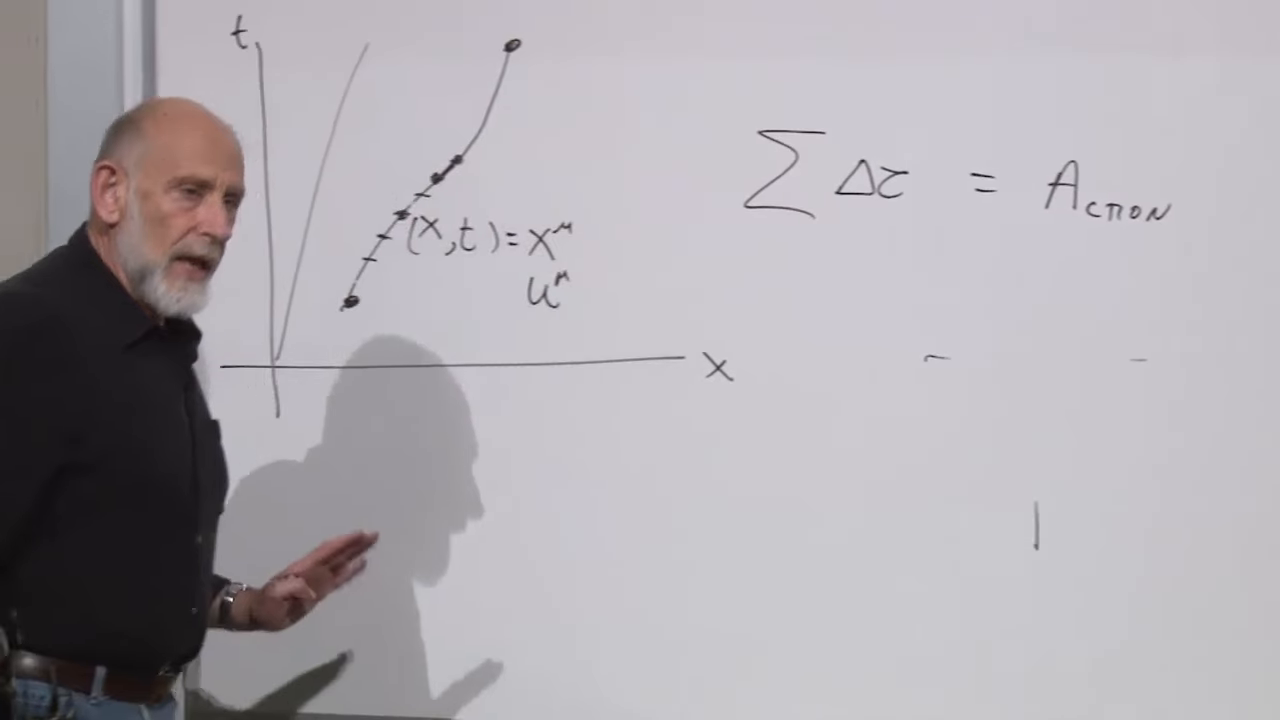
\includegraphics[width=0.90\textwidth]{lecture_03_figure_09.png}
\caption{作用量是沿端点固定的变分世界线对不变固有时增量的求和。}
\lectureframe{00:38:30}
\end{figure}

\begin{classroomqa}
\audiencequestion{如果作用量乘以一个任意常数，能量会怎样？}
\lecturerresponse{能量不是起始的不变量；它将从拉格朗日量和哈密顿量导出。将整个作用量乘以一个非零常数不会改变其驻值路径，尽管它会重新标度由该作用量定义的正则量。选择归一化 \(-m\) 是为了使这些导出的量与既有的牛顿约定相符。\lecturetimestamp{00:39:47}}
\end{classroomqa}

\begin{classroomqa}
\audiencequestion{为什么像固有时这样的不变量是构造作用量的良好候选？}
\lecturerresponse{因为稳定作用量定律应当在每个惯性系中选出相同的物理路径。这类似于在欧几里得平面中寻找最短曲线：旋转改变坐标分量，但不改变每个无穷小长度，因此它们不能改变哪条曲线最短。用固有时替换欧几里得长度，就给出了相对论性的构造。\lecturetimestamp{00:40:39}}
\end{classroomqa}

\begin{classroomqa}
\audiencequestion{为什么固有时选择正平方根而不是负平方根？}
\lecturerresponse{固有时被定义为从过去到未来携带的时钟的正的流逝读数。一致地选择负平方根只会反转作用量的符号，把最小值变成最大值，而不改变稳定世界线。在时钟的静止系中，正号约定给出\(d\tau=dt\)。\lecturetimestamp{00:42:59}}
\end{classroomqa}

因子\(-m\)同样是为了恢复牛顿力学而选定的归一化约定。恢复单位后，传统作用量为
\begin{equation}
S=-mc^2\int_a^b d\tau.
\label{eq:sr3-action-dimensional}
\end{equation}

\begin{figure}[htbp]
\centering
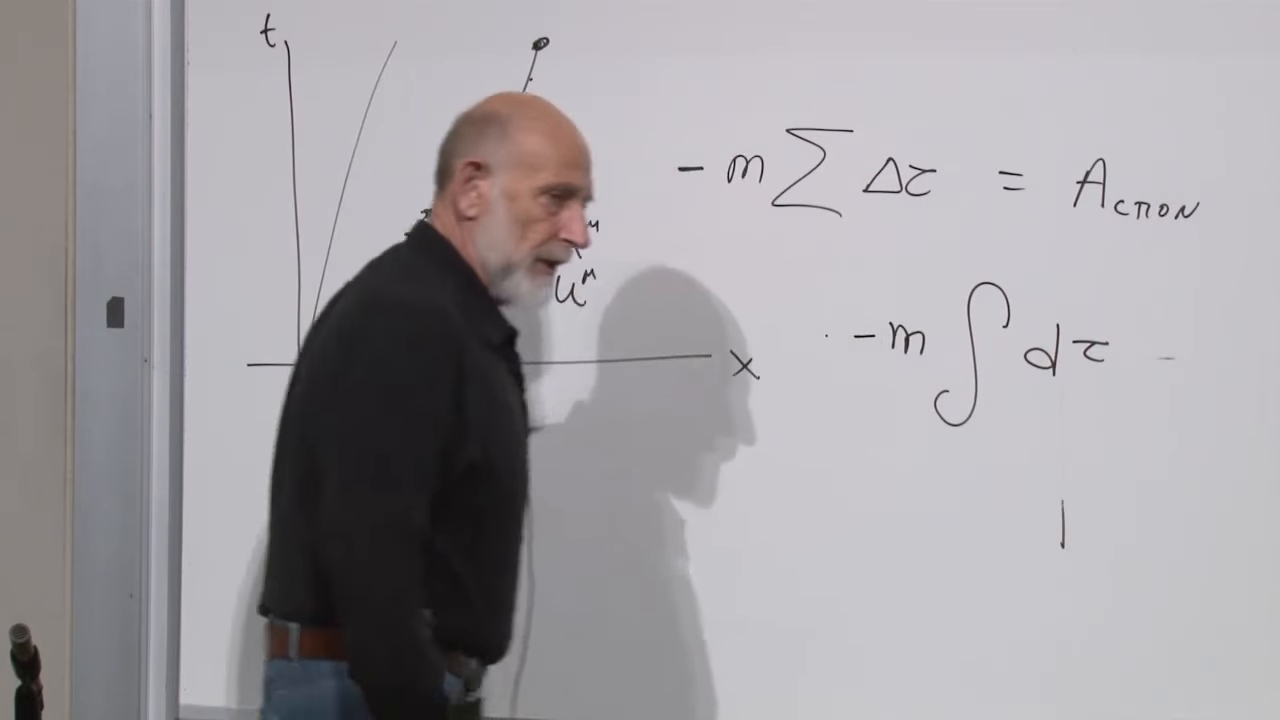
\includegraphics[width=0.90\textwidth]{lecture_03_figure_10.png}
\caption{在自然单位下，有限固有时的求和变成不变量积分\(-m\int d\tau\)。}
\lectureframe{00:46:23}
\end{figure}

\section{相对论拉格朗日量}

为了把作用量写成标准力学形式，从\(d\tau\)中提出因子\(dt\)：
\begin{equation}
d\tau
=dt\sqrt{1-\dot{\vec x}^{\,2}},
\qquad
\dot{\vec x}^{\,2}
=\dot x^2+\dot y^2+\dot z^2.
\end{equation}
于是
\begin{equation}
S
=
\int_a^b L\,dt,
\qquad
\boxed{
L=-m\sqrt{1-v^2}
}
\quad(c=1).
\label{eq:sr3-relativistic-lagrangian}
\end{equation}
在传统单位中，
\begin{equation}
L=-mc^2\sqrt{1-\frac{v^2}{c^2}}.
\label{eq:sr3-relativistic-lagrangian-c}
\end{equation}
这是自由粒子的拉格朗日量：它依赖于速度，但不依赖于位置。尚未引入任何力或势。

\begin{figure}[htbp]
\centering
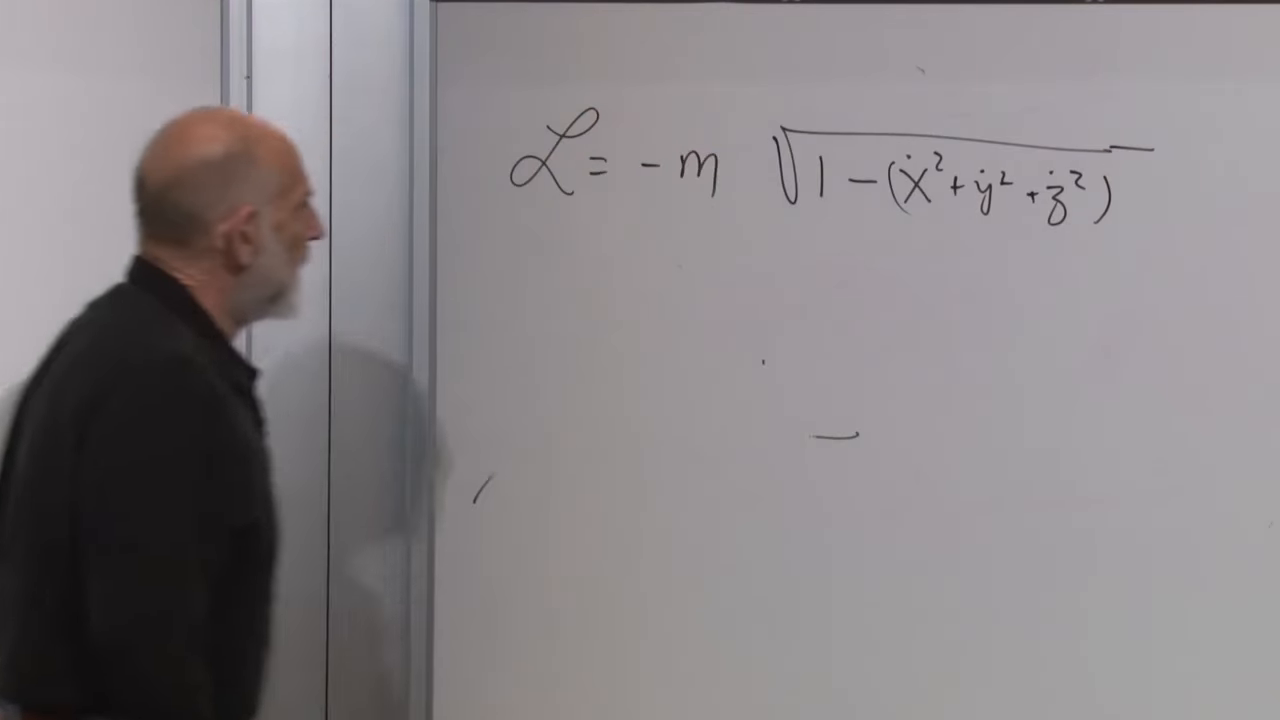
\includegraphics[width=0.90\textwidth]{lecture_03_figure_11.png}
\caption{提出\(dt\)后，可以看出自由相对论拉格朗日量是三个速度分量的函数。}
\lectureframe{00:49:57}
\end{figure}

\subsection{恢复拉格朗日与牛顿}

代入\eqref{eq:sr3-sqrt-expansion}：
\begin{align}
L
&=-m\sqrt{1-v^2}\\
&\approx-m\left(1-\frac{v^2}{2}\right)\\
&=-m+\frac12mv^2.
\label{eq:sr3-lagrangian-low-speed}
\end{align}
常数\(-m\)既不依赖于位置，也不依赖于速度。它对具有相同端点时间的每条路径贡献相同的量，因此从欧拉--拉格朗日方程中消失。具有动力学内容的部分正是
\begin{equation}
L_{\mathrm{Newton}}=\frac12mv^2.
\end{equation}
因此，不变量作用量中的符号和质量归一化被正确地选定了。

\begin{figure}[htbp]
\centering
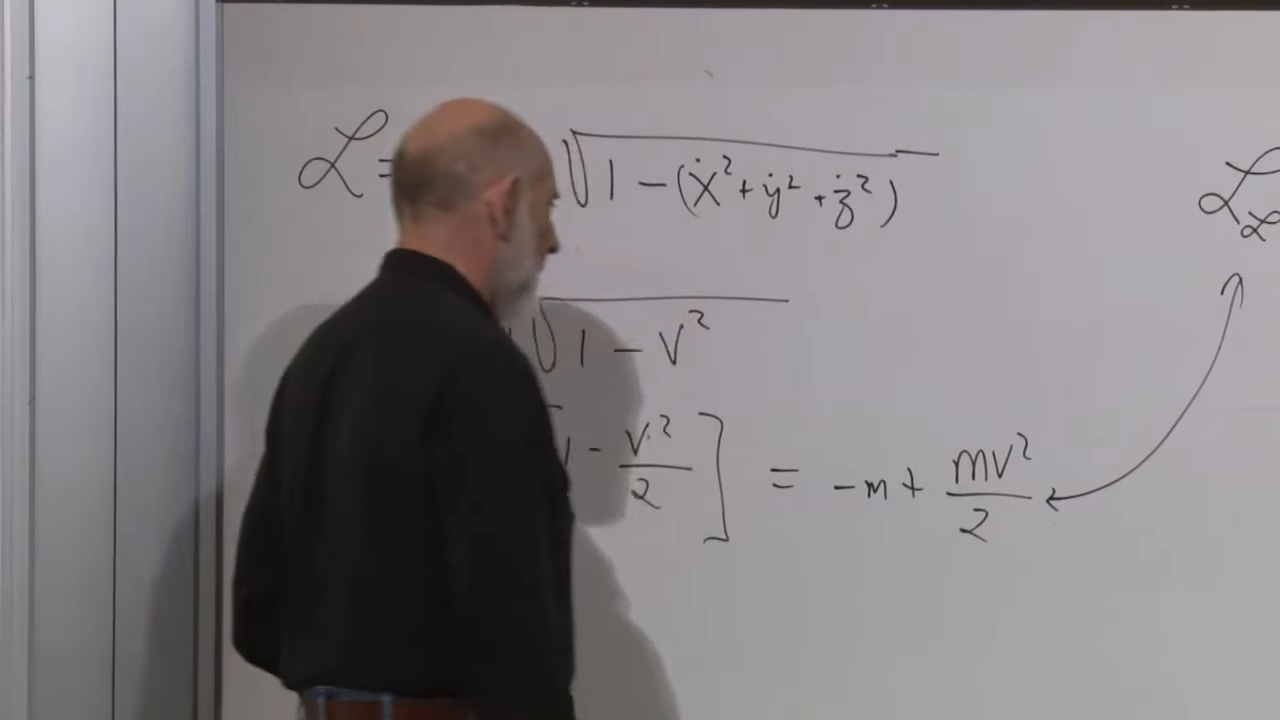
\includegraphics[width=0.90\textwidth]{lecture_03_figure_12.png}
\caption{低速展开留下一个常数\(-m\)和牛顿自由粒子拉格朗日量\(mv^2/2\)。}
\lectureframe{00:53:24}
\end{figure}

对于目前的自由粒子，欧拉--拉格朗日方程只会说明速度是常数，并且时空世界线是直线。更有启发性的任务是识别守恒的动量和能量。

\section{正则动量}

因为\(L\)不依赖于位置，所以它在空间平移下不变。相应的守恒量是动量。我们不假设牛顿公式\(p_i=mv_i\)；我们使用正则定义
\begin{equation}
p_i=\frac{\partial L}{\partial\dot x^i}.
\label{eq:sr3-canonical-momentum}
\end{equation}
对于\(L=-m\sqrt{1-v^2}\)，
\begin{align}
p_i
&=
-m\frac{1}{2\sqrt{1-v^2}}
\frac{\partial}{\partial\dot x^i}(1-v^2)\\
&=
-m\frac{1}{2\sqrt{1-v^2}}(-2\dot x^i)\\
&=
\frac{mv_i}{\sqrt{1-v^2}}
=m\gamma v_i.
\label{eq:sr3-relativistic-momentum}
\end{align}
由于\(u^i=\gamma v^i\)，
\begin{equation}
\boxed{
p^i=mu^i
}.
\label{eq:sr3-momentum-spatial}
\end{equation}
在低速下，这约化为\(p^i\approx mv^i\)。在接近光速时，分母起决定性作用。

\begin{figure}[htbp]
\centering
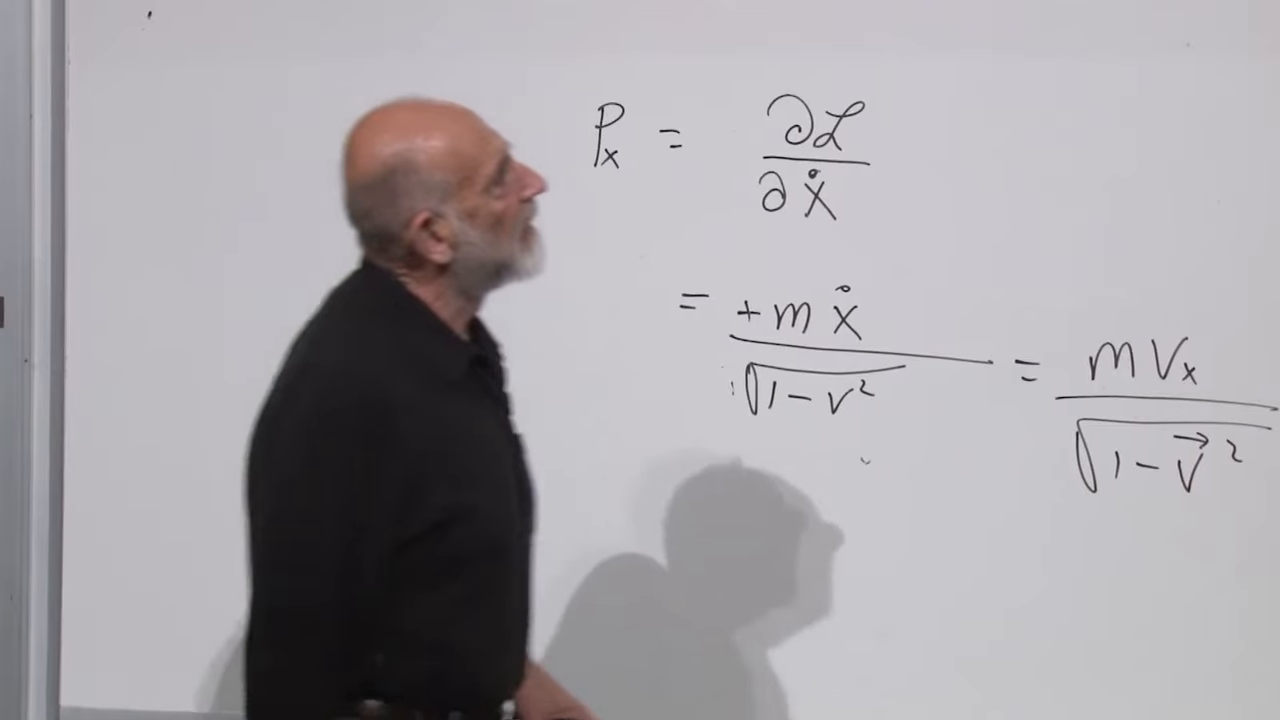
\includegraphics[width=0.90\textwidth]{lecture_03_figure_13.png}
\caption{对平方根拉格朗日量作正则微分给出\(p_x=mv_x/\sqrt{1-v^2}\)。}
\lectureframe{00:58:49}
\end{figure}

\subsection{质量，而非相对论质量}

这里的\(m\)就是粒子的质量：一个不变量标签，当粒子运动时不会改变。较早的文献有时称它为\emph{静质量}，并称\(E/c^2\)为依赖于速度的\emph{相对论质量}。现代用法避免这种区分。运动改变能量和动量，而不改变不变量质量。电子在任何参考系中都具有相同的质量参数。

\section{从三维动量到四维动量}

关于四维矢量某一个分量的陈述通常是依赖于参考系的。例如，\(\Delta\vec x=0\)表示两个事件在一个参考系中具有相同的位置，但一个推动会使该间隔倾斜，并使得\(\Delta\vec x'\ne0\)。相比之下，
\begin{equation}
\Delta x^\mu=0
\end{equation}
是不变量：如果所有四个分量在一个参考系中为零，那么在所有参考系中所有四个分量都为零。同样，\(\vec u=0\)只标识粒子的静止系；它不是对四维速度的不变量描述。

对于封闭系统，普通动量守恒写作
\begin{equation}
\vec P_{\mathrm{initial}}-\vec P_{\mathrm{final}}=0.
\label{eq:sr3-three-momentum-conservation}
\end{equation}
这是一个三维矢量方程。为了使守恒明显地洛伦兹协变，我们需要一个第四分量来与三个\(p^i=mu^i\)结合。显然的补全是
\begin{equation}
p^\mu=mu^\mu.
\label{eq:sr3-four-momentum}
\end{equation}
在\(c=1\)单位下，
\begin{equation}
p^\mu=(p^0,\vec p)
=
m\gamma(1,\vec v).
\end{equation}

\begin{figure}[htbp]
\centering
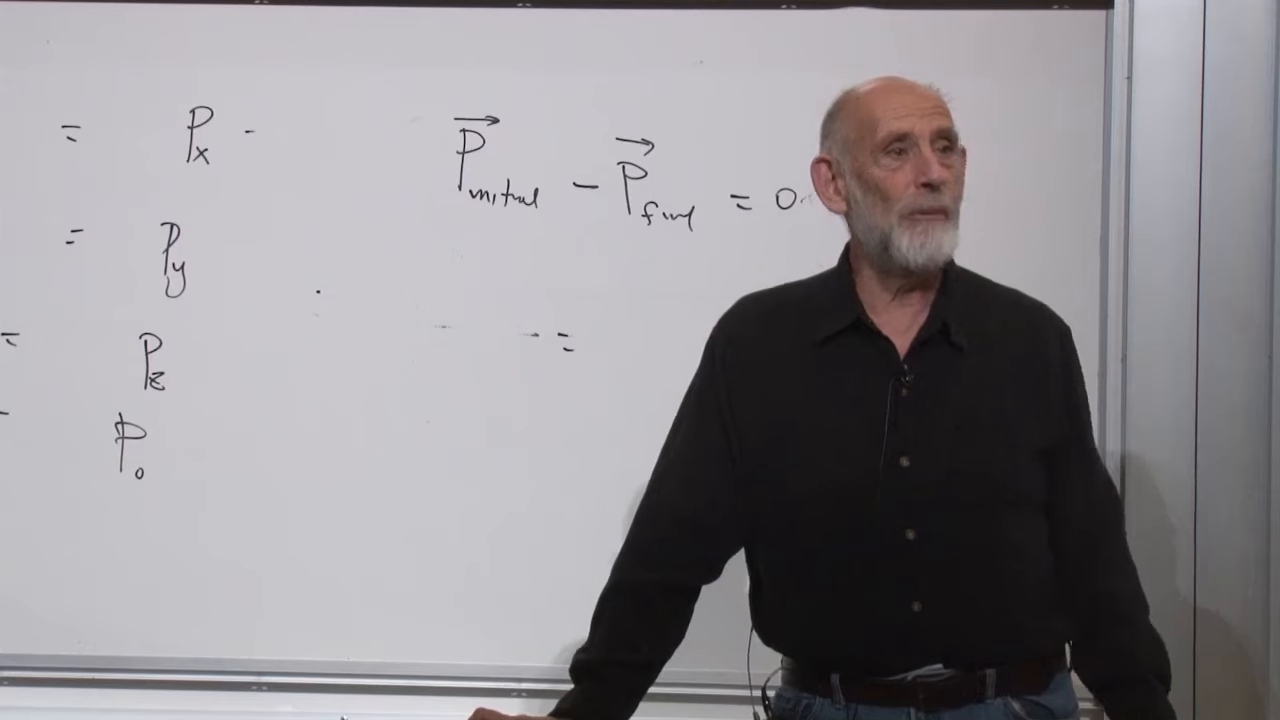
\includegraphics[width=0.90\textwidth]{lecture_03_figure_14.png}
\caption{只有在空间分量由一个第四分量补全之后，动量守恒才成为不变量。}
\lectureframe{01:09:51}
\end{figure}

缺失的分量本身必须守恒。粒子力学中已经包含另一个守恒量：能量。问题在于，\(p^0=mu^0=m\gamma\) 在自然单位制下是否恰好就是那个能量。系统的回答来自哈密顿量。

\section{哈密顿量就是能量}

对于任何这种形式的、不显含时间的拉格朗日量，哈密顿量为
\begin{equation}
H=\sum_{i=1}^{3}\dot x^i p_i-L.
\label{eq:sr3-hamiltonian-definition}
\end{equation}
这个公式并非牛顿力学所特有。它是从速度到正则动量的通用勒让德变换，同样适用于相对论性拉格朗日量。

\begin{figure}[htbp]
\centering
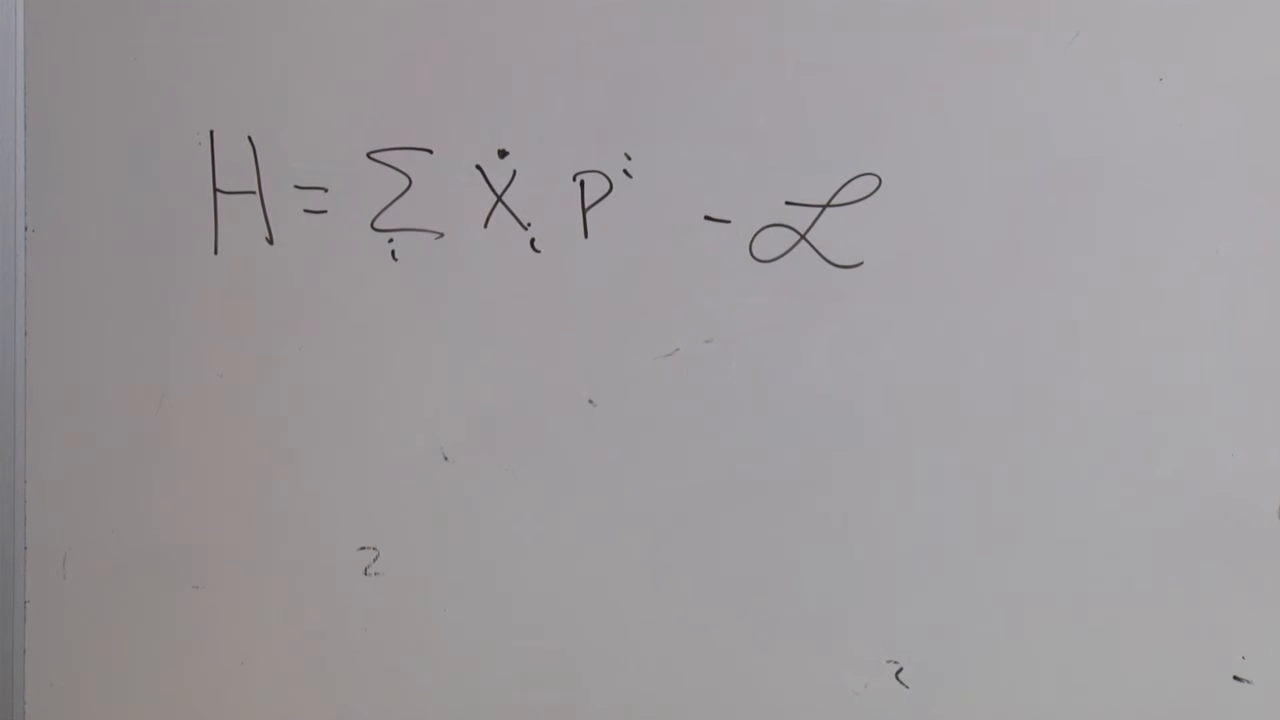
\includegraphics[width=0.90\textwidth]{lecture_03_figure_15.png}
\caption{一般的哈密顿量公式 \(H=\sum_i\dot x^i p_i-L\)。}
\lectureframe{01:11:55}
\end{figure}

代入 \(p_i=m\dot x_i/\sqrt{1-v^2}\) 和 \(L=-m\sqrt{1-v^2}\)：
\begin{align}
H
&=
\frac{mv^2}{\sqrt{1-v^2}}
+m\sqrt{1-v^2}\\
&=
\frac{mv^2+m(1-v^2)}{\sqrt{1-v^2}}\\
&=
\boxed{\frac{m}{\sqrt{1-v^2}}}
=m\gamma.
\label{eq:sr3-hamiltonian-result}
\end{align}
相消是关键步骤。与 \(u^0=\gamma\) 比较，
\begin{equation}
H=mu^0=p^0.
\end{equation}
因此第四分量就是能量：
\begin{equation}
p^\mu=(E,\vec p),
\qquad
E=H
\qquad(c=1).
\label{eq:sr3-four-momentum-natural}
\end{equation}

\begin{figure}[htbp]
\centering
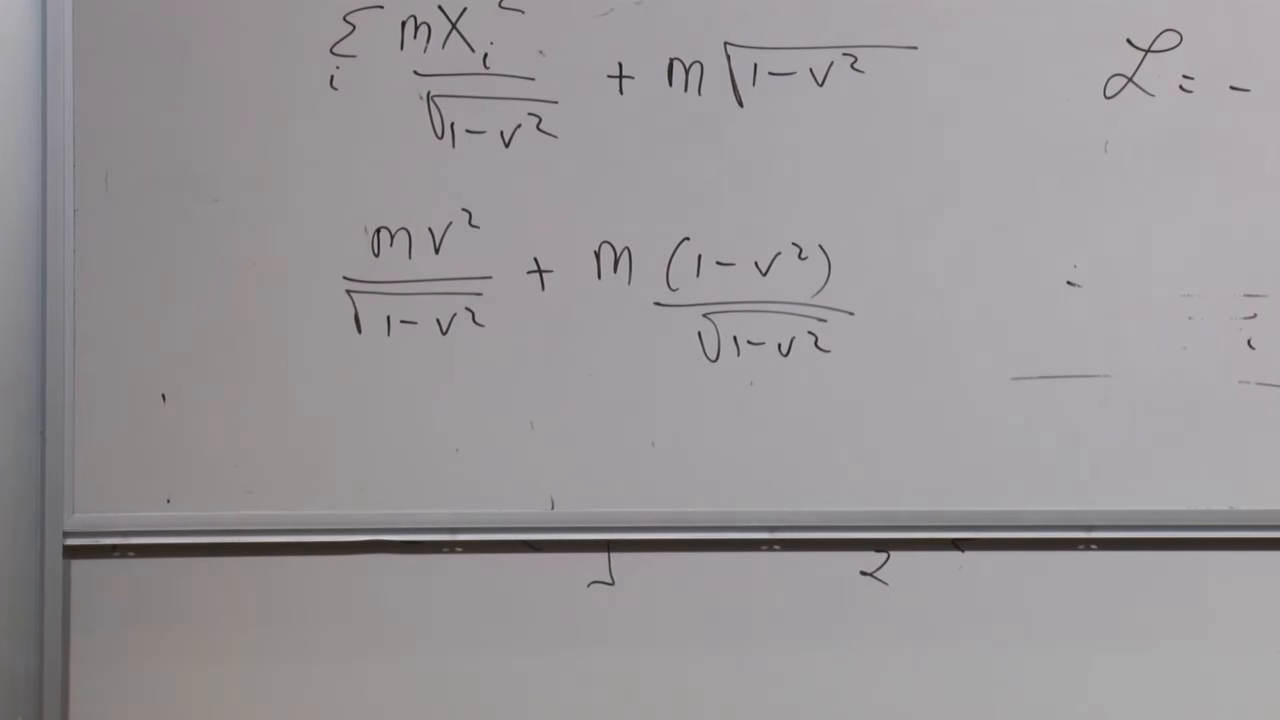
\includegraphics[width=0.90\textwidth]{lecture_03_figure_16.png}
\caption{哈密顿量中的两项通分合并；\(mv^2\) 的贡献相消。}
\lectureframe{01:14:28}
\end{figure}

\begin{classroomqa}
\audiencequestion{公式 \(H=\sum_i\dot x^i p_i-L\) 只是经典力学的哈密顿量公式吗？}
\lecturerresponse{它是与拉格朗日量相联系的通用勒让德变换，而不是某种特殊的非相对论假设。\(L\) 的形式决定了得到哪种力学结果。在这里，相对论性的平方根拉格朗日量给出 \(H=m/\sqrt{1-v^2}\)。\lecturetimestamp{01:15:21}}
\end{classroomqa}

不变量形式的守恒陈述现在为
\begin{equation}
\sum_{\mathrm{initial}}p^\mu
=
\sum_{\mathrm{final}}p^\mu,
\label{eq:sr3-four-momentum-conservation}
\end{equation}
它把能量守恒和动量的全部三个分量包含在一个四维矢量方程中。

\section{静能与牛顿极限}

在自然单位制下，精确能量为
\begin{equation}
E=\frac{m}{\sqrt{1-v^2}}.
\end{equation}
利用 \eqref{eq:sr3-gamma-expansion}，
\begin{equation}
E
\approx
m+\frac12mv^2+\frac38mv^4+\cdots .
\label{eq:sr3-energy-natural-expansion}
\end{equation}
第二项是熟悉的动能。第一项是质心静止时仍然保留的能量。

\begin{figure}[htbp]
\centering
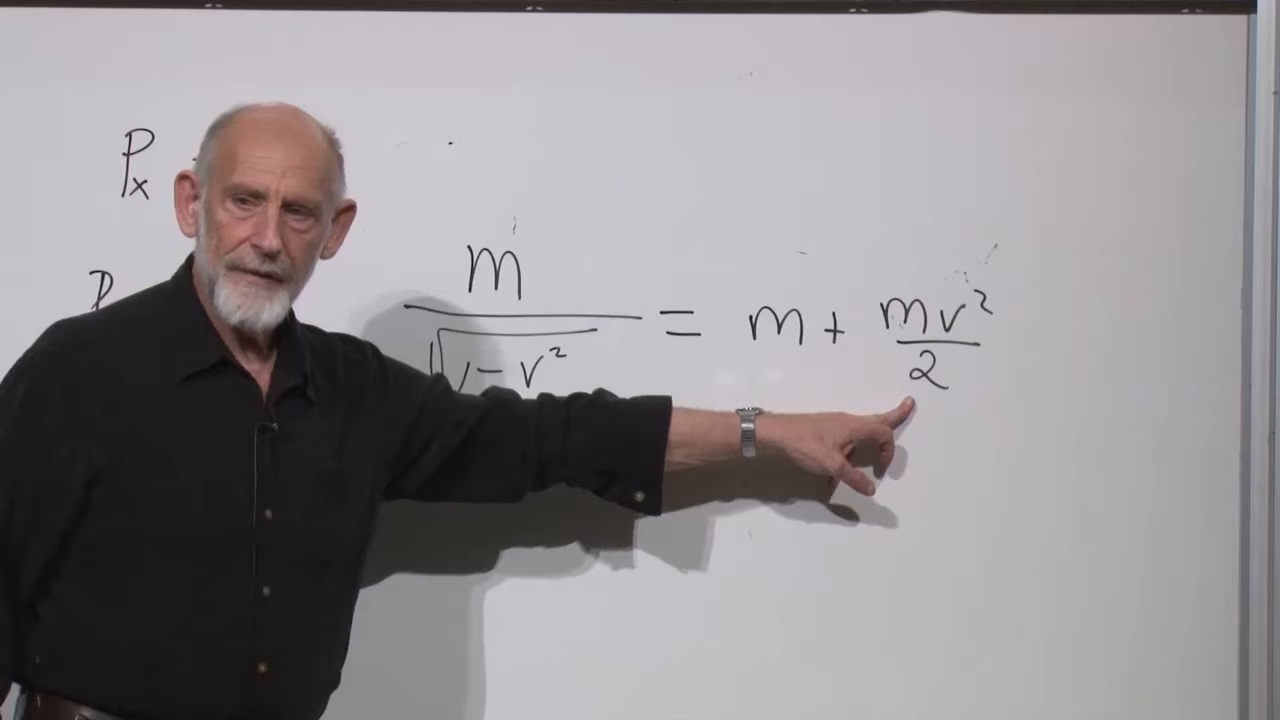
\includegraphics[width=0.90\textwidth]{lecture_03_figure_17.png}
\caption{精确能量在单位 \(c=1\) 下展开为 \(m+mv^2/2+\cdots\)。}
\lectureframe{01:18:02}
\end{figure}

在精确表达式中恢复量纲。平方根内的比值必须是 \(v^2/c^2\)，而分子必须具有能量的量纲：
\begin{equation}
\boxed{
E
=
\gamma mc^2
=
\frac{mc^2}{\sqrt{1-v^2/c^2}}
}.
\label{eq:sr3-energy-exact}
\end{equation}
其低速展开为
\begin{equation}
\boxed{
E
=
mc^2+\frac12mv^2
+\frac38m\frac{v^4}{c^2}
+\cdots
}.
\label{eq:sr3-energy-dimensional-expansion}
\end{equation}
静止时，
\begin{equation}
\boxed{E_{\mathrm{rest}}=mc^2}.
\label{eq:sr3-emc2}
\end{equation}

\begin{figure}[htbp]
\centering
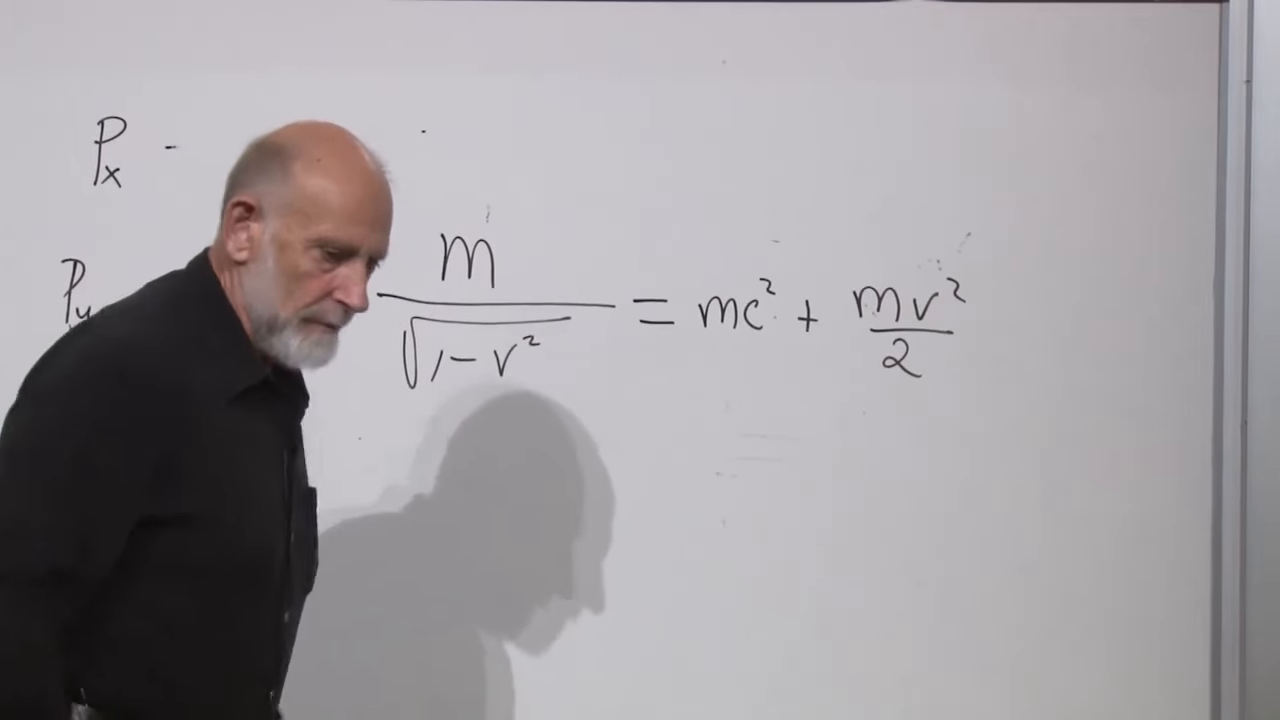
\includegraphics[width=0.90\textwidth]{lecture_03_figure_18.png}
\caption{量纲恢复把常数项变为 \(mc^2\)，其后是牛顿动能 \(mv^2/2\)。}
\lectureframe{01:19:16}
\end{figure}

这适用于任何封闭物体，而不仅限于基本粒子。\emph{静止} 意味着质心静止。物体内部的分子、原子和场仍然可以运动和相互作用。它们的内动能、势能和结合能都对总静能有贡献，因而也对物体的不变质量有贡献。

\begin{classroomqa}
\audiencequestion{转换因子会不会是 \(c^2\) 除以某个任意数？}
\lecturerresponse{仅凭量纲就能确定 \(c\) 的幂次，但系数由自然单位制的结果固定。普通单位制下的公式在 \(c=1\) 时必须约化为 \(E=m\)，所以恢复量纲后的表达式在静止时为 \(E=mc^2\)，系数为一。\lecturetimestamp{01:22:08}}
\end{classroomqa}

\begin{classroomqa}
\audiencequestion{二项式展开中的首项一在物理上重要吗？更高阶的项又意味着什么？}
\lecturerresponse{是的。在能量展开中，首项一变为静能 \(mc^2\)。下一项是牛顿动能，而所有更高阶的项都是相对论修正。对于棒球来说它们可以忽略，但当 \(v\) 趋近 \(c\) 时它们就变得必不可少。\lecturetimestamp{01:22:37}}
\end{classroomqa}

当 \(v\to c\) 时，精确的能量和动量都发散：
\begin{equation}
\begin{aligned}
E&=\gamma mc^2\longrightarrow\infty,\\
\vec p&=\gamma m\vec v\longrightarrow\infty
\qquad(m>0).
\end{aligned}
\end{equation}
因此，达到光速将需要无限大的能量和动量。有限大小的力在有限时间内只提供有限的冲量，所以有质量的粒子可以趋近 \(c\)，但无法达到它。

\begin{classroomqa}
\audiencequestion{现在是什么在强制光速壁垒？}
\lecturerresponse{精确的四维动量在强制它。当有质量的粒子趋近 \(c\) 时，能量和动量都发散，而四维动量守恒约束着每一次相互作用。先前对四维速度的归一化是同一陈述的运动学形式。\lecturetimestamp{01:24:27}}
\end{classroomqa}

\section{复合系统的质量}

假设两个粒子以大小相等、方向相反的动量运动。它们的总三维动量为零，因此我们已经处在复合系统的静止系中。该系统的\(M\)不变质量由它在此系中的总能量定义：
\begin{equation}
Mc^2=E_{\mathrm{tot}}
\qquad
(\vec P_{\mathrm{tot}}=0).
\end{equation}
更一般地，
\begin{equation}
M^2c^4
=
E_{\mathrm{tot}}^2-c^2\vec P_{\mathrm{tot}}^{\,2}.
\label{eq:sr3-composite-mass}
\end{equation}

\begin{classroomqa}
\audiencequestion{对于两个沿相反方向运动的粒子，组合系统的质量是否大于它们各自质量之和？}
\lecturerresponse{如果它们是自由的，是的：在动量中心系中，它们的动能加到总静止能量上，因此\(M>m_1+m_2\)。吸引性的束缚能反而可以降低总能量，给出\(M<m_1+m_2\)。不变定义是在总动量为零的参考系中的总能量。\lecturetimestamp{01:25:06}}
\end{classroomqa}

这就是为什么在称量一个复合物体时，内部运动和束缚不能忽略。不变质量属于整个封闭系统，而不只是各组成粒子质量的简单算术列表。

\begin{classroomqa}
\audiencequestion{静止能量项在量子态的相位中起什么作用？}
\lecturerresponse{具有确定能量的态以相位\(\exp(-iEt/\hbar)\)演化，因此静止的粒子贡献\(\exp(-imc^2t/\hbar)\)。共同的总体相位不可观测，但具有不同能量的各分量之间的相对相位可以观测。这一量子后果与这里的经典推导一致，但并非经典推导所必需。\lecturetimestamp{01:26:57}}
\end{classroomqa}

\section{能量--动量关系}

四维速度的归一化立即给出四维动量的不变模长。在\(c=1\)单位下，
\begin{equation}
(u^0)^2-\vec u^{\,2}=1.
\end{equation}

乘以\(m^2\)并利用\(p^\mu=mu^\mu\)，
\begin{equation}
\boxed{
E^2-\vec p^{\,2}=m^2
}
\qquad(c=1).
\label{eq:sr3-mass-shell-natural}
\end{equation}
等价地，
\begin{equation}
E=\sqrt{\vec p^{\,2}+m^2}.
\end{equation}

\begin{figure}[htbp]
\centering
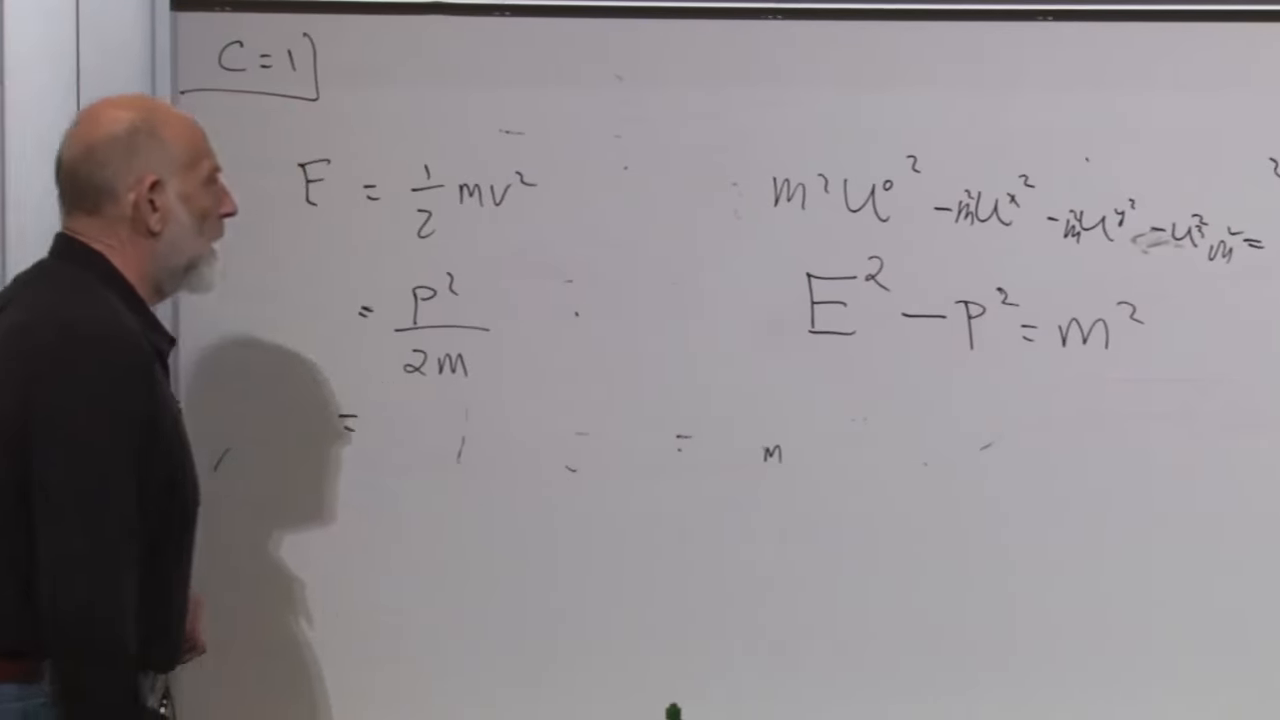
\includegraphics[width=0.90\textwidth]{lecture_03_figure_19.png}
\caption{将四维速度归一化式乘以\(m^2\)得到\(E^2-\vec p^{\,2}=m^2\)。}
\lectureframe{01:31:48}
\end{figure}

恢复\(c\)，
\begin{equation}
\boxed{
E^2
=
\vec p^{\,2}c^2+m^2c^4
},
\qquad
E=\sqrt{\vec p^{\,2}c^2+m^2c^4}.
\label{eq:sr3-mass-shell}
\end{equation}
这个公式将能量表示为动量的函数，而不涉及速度。它是牛顿关系式
\begin{equation}
K=\frac{\vec p^{\,2}}{2m}.
\end{equation}的相对论类比。

\begin{figure}[htbp]
\centering
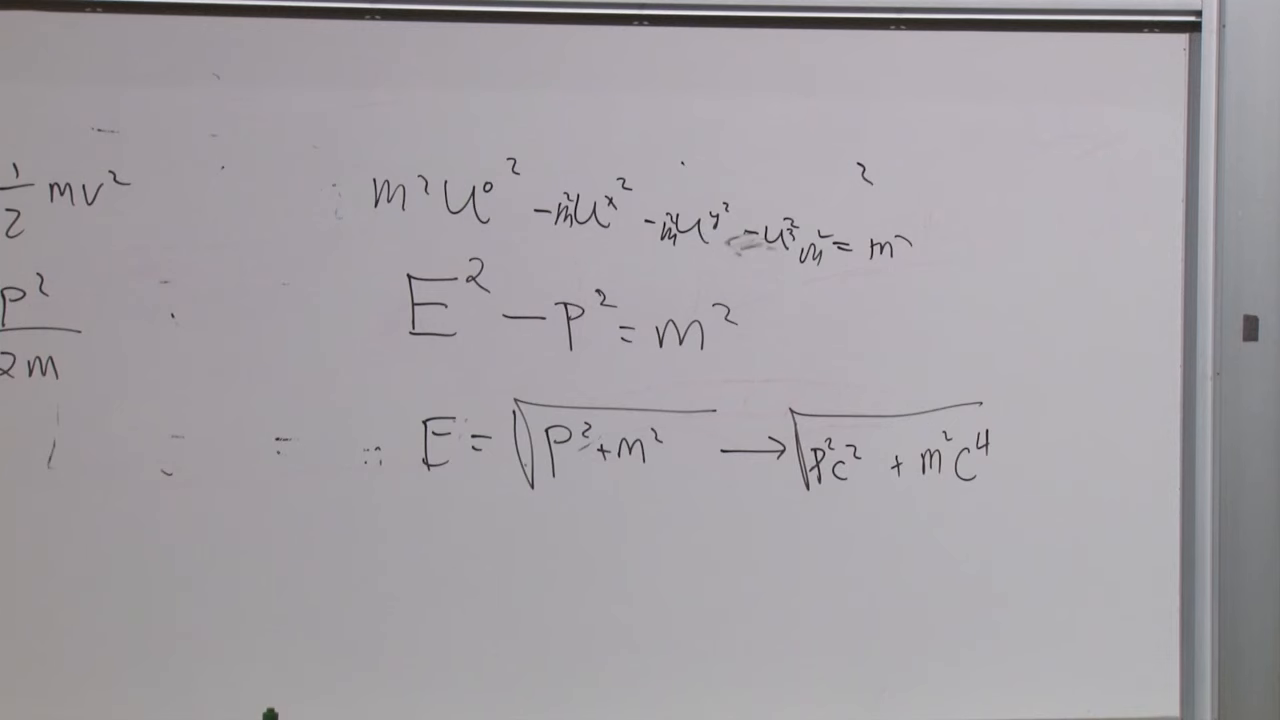
\includegraphics[width=0.90\textwidth]{lecture_03_figure_20.png}
\caption{恢复量纲后的质量壳关系：\(E=\sqrt{\vec p^{\,2}c^2+m^2c^4}\)。}
\lectureframe{01:32:38}
\end{figure}

\subsection{无质量粒子}

速度公式\(E=\gamma mc^2\)在\(m=0\)且\(v=c\)时成为不确定的\(0/0\)形式。因此速度不是区分无质量粒子的好标签：真空中每一个自由传播的无质量粒子都以\(c\)运动，然而不同的光子可以有不同的能量。

能量--动量关系有一个光滑的无质量极限：
\begin{equation}
m=0
\quad\Longrightarrow\quad
\boxed{E=c|\vec p|}.
\label{eq:sr3-massless-energy}
\end{equation}
这适用于光子，在理想化的无质量理论中也适用于引力子。只要\(mc^2\ll E\)，它就是对高度相对论性粒子的极好近似，包括能量足够高的中微子，尽管它们具有很小的非零质量。

\begin{figure}[htbp]
\centering
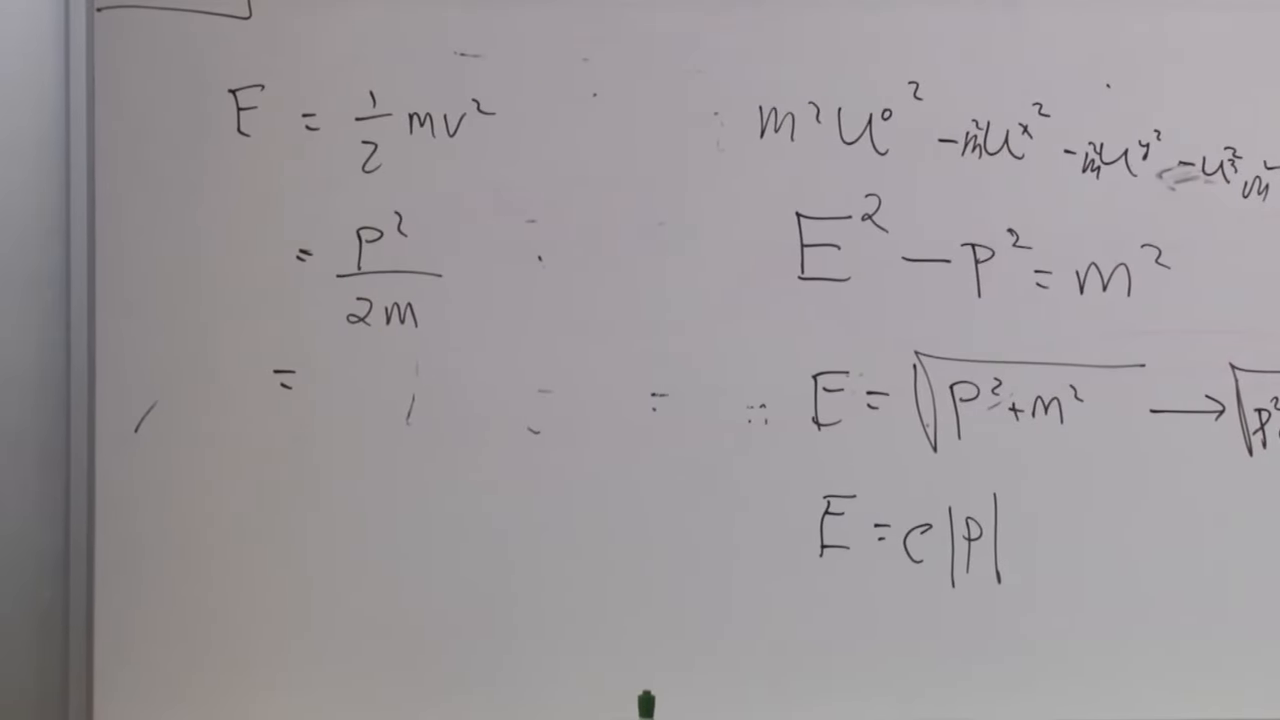
\includegraphics[width=0.90\textwidth]{lecture_03_figure_21.png}
\caption{能量--动量关系的无质量极限给出\(E=c|\vec p|\)。}
\lectureframe{01:33:48}
\end{figure}

\section{电子偶素衰变}

考虑电子偶素，即电子和正电子的束缚态。它的不变质量略小于\(2m_e\)：各组成粒子具有正的内部动能，但具有更大的负束缚能。数值上，
\begin{equation}
m_ec^2\approx0.511\ \mathrm{MeV},
\qquad
m_e\approx9.11\times10^{-31}\ \mathrm{kg},
\end{equation}
但运动学并不依赖于这个数值。

取电子偶素静止系中的双光子衰变道：
\begin{equation}
\mathrm{Ps}\longrightarrow\gamma+\gamma.
\end{equation}
初始时总动量为零。因此动量守恒要求两个光子以大小相等、方向相反的动量背对背出射：
\begin{equation}
\vec p_1=\vec p,
\qquad
\vec p_2=-\vec p.
\label{eq:sr3-positronium-momentum}
\end{equation}
若\(M\)是电子偶素质量，能量守恒给出
\begin{equation}
Mc^2
=E_1+E_2
=c|\vec p_1|+c|\vec p_2|
=2c|\vec p|.
\end{equation}
因此
\begin{equation}
\boxed{
|\vec p|=\frac{Mc}{2},
\qquad
E_1=E_2=\frac{Mc^2}{2}
}.
\label{eq:sr3-positronium-result}
\end{equation}

\begin{figure}[htbp]
\centering
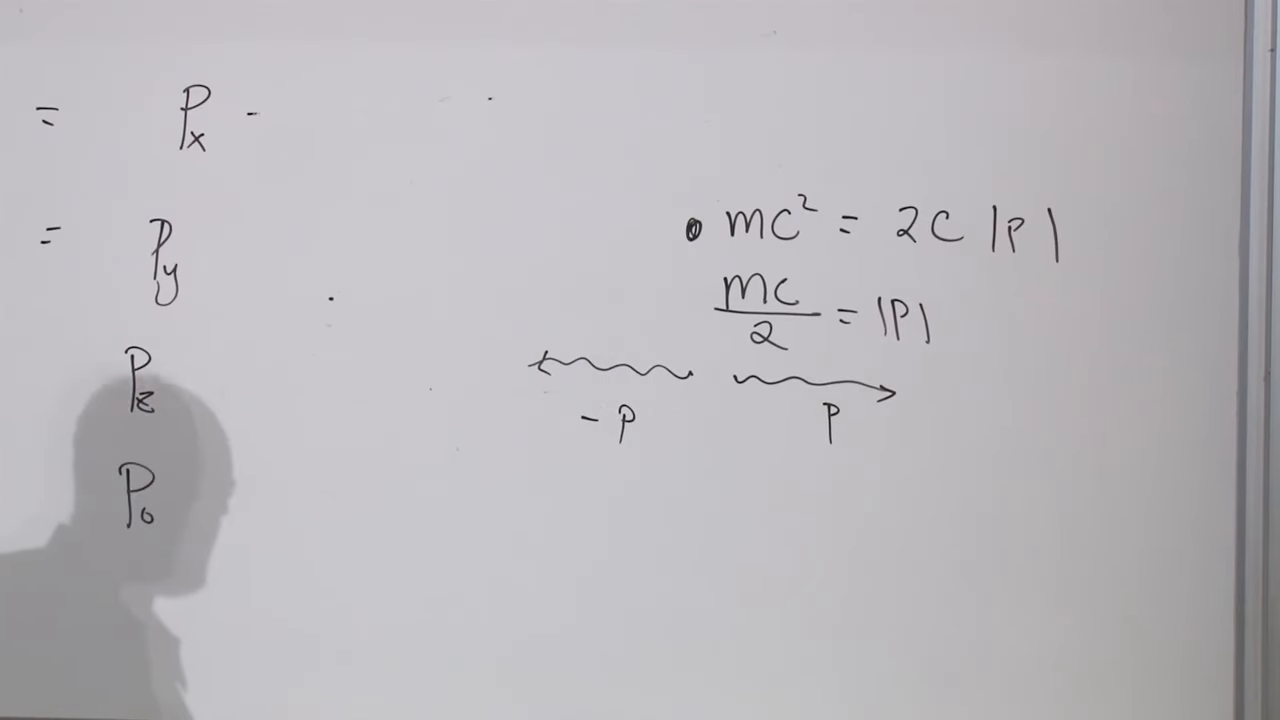
\includegraphics[width=0.90\textwidth]{lecture_03_figure_22.png}
\caption{静止的电子偶素态衰变为两个动量大小相等、方向相反的光子；\(Mc^2=2c|\vec p|\)。}
\lectureframe{01:40:55}
\end{figure}

这个过程没有粒子质量之和守恒的牛顿类比。入射态具有非零不变质量，而每个出射光子都是无质量的。守恒的是总四维动量。储存的静止能量已变成传播的电磁能量。利用量子关系\(|\vec p|=h/\lambda\)，同一结果确定了光子波长；相应的光子能量远高于光学范围。

\begin{classroomqa}
\audiencequestion{衰变中角动量如何守恒？}
\lecturerresponse{出射辐射必须携带与初始态相同的总角动量。在双光子道中，光子螺旋度和它们的轨道态以适当方式组合。更精确地说，自旋单态的仲电子偶素主要衰变为两个光子，而自旋三重态的 ortho-positronium 主要衰变为三个；允许的道尊重所有量子数。\lecturetimestamp{01:42:11}}
\end{classroomqa}

\begin{classroomqa}
\audiencequestion{为什么以光速运动的粒子必须是无质量的？}
\lecturerresponse{对于有限非零能量，因子\(\gamma\)在\(v\to c\)时发散。不变关系式\(E^2-\vec p^{\,2}c^2=m^2c^4\)表明，四动量为零的粒子满足\(m=0\)。反之，自由无质量粒子具有零世界线，并以\(c\)传播。\lecturetimestamp{01:42:50}}
\end{classroomqa}

\begin{classroomqa}
\audiencequestion{同一个中性态能否不衰变为光子而衰变为引力子？}
\lecturerresponse{原则上，当量子数允许时，引力末态是允许的，但引力分支比电磁分支比小得不可思议。运动学上的记账仍将使用相同的四动量守恒以及每个无质量量子的\(E=c|\vec p|\)。\lecturetimestamp{01:43:20}}
\end{classroomqa}

\subsection{一个衰变顶点}

衰变是局域的：母粒子世界线终止于一个时空事件，出射光子的世界线从该事件开始。探测器相互作用可以反向外推以重建那个共同顶点。如果两个光子是在不同事件发射的，它们反向外推的零轨迹就不会交于一点。

\begin{classroomqa}
\audiencequestion{两个光子是否必须在所有参考系中同时发射？}
\lecturerresponse{它们起源于同一个时空事件，而不是两个空间上分离、其同时性可能依赖于参考系的事件。所有洛伦兹参考系都同意一个事件就是一个事件。量子力学赋予母粒子有限的位置不确定度，因此重建的顶点是一个分布，而不是一个完全已知的经典点。\lecturetimestamp{01:44:01}}
\end{classroomqa}

\begin{classroomqa}
\audiencequestion{为什么四速度的模等于一？}
\lecturerresponse{固有时由\(d\tau^2=dt^2-d\vec x^{\,2}\)在单位\(c=1\)下定义。除以\(d\tau^2\)得到\((dt/d\tau)^2-(d\vec x/d\tau)^2=1\)，这恰好就是\((u^0)^2-\vec u^{\,2}=1\)。因此归一化已内建于固有时定义之中。\lecturetimestamp{01:45:38}}
\end{classroomqa}

\begin{classroomqa}
\audiencequestion{\(u^0=dt/d\tau\)是否给出了对能量的更深层解释？}
\lecturerresponse{它给出了有用的恒等式\(E=mc^2\,dt/d\tau=\gamma mc^2\)：静止时坐标时与固有时之比为一，运动时则为洛伦兹因子。除了编码这种速度依赖性之外，该恒等式本身并不增添独立的动力学原理。\lecturetimestamp{01:46:36}}
\end{classroomqa}

\section{守恒要求一个封闭系统}

陈述
\begin{equation}
\sum p^\mu_{\mathrm{initial}}
=
\sum p^\mu_{\mathrm{final}}
\end{equation}
适用于一个包含所有交换能量和动量的东西的孤立系统。真实实验室中存在杂散电场和磁场、环境粒子、引力、支撑物和探测器。如果把这些自由度留在记账之外，子系统就可能显示出微小的表观不平衡；缺失的四动量已进入环境。

\begin{classroomqa}
\audiencequestion{双光子动量之和是否可能是一个与零有微小差异的量？}
\lecturerresponse{对于完整的孤立系统而言不会。在实际实验中，未被建模的场或装置的反冲可以携带那微小的余量，因此所选子系统可能看起来并不封闭。一旦把所有相互作用的部件都包括进来，总四动量就是守恒的。\lecturetimestamp{01:47:51}}
\end{classroomqa}

\begin{classroomqa}
\audiencequestion{不确定性原理会削弱动量守恒吗？}
\lecturerresponse{不会。量子态可以具有不确定的位置或动量，而对其中一个知道得越精确就会使另一个的分布越宽，但对于孤立系统，平移对称性仍然给出总动量的精确守恒。量子不确定性关乎结果和分布，而不是守恒定律的失效。\lecturetimestamp{01:49:19}}
\end{classroomqa}

\section{精确能量与近似能量}

重要的是不要把精确公式与其低速展开相混淆：
\begin{align}
E_{\mathrm{exact}}
&=
\frac{mc^2}{\sqrt{1-v^2/c^2}},
\label{eq:sr3-exact-repeated}\\
E_{\mathrm{slow}}
&=
mc^2+\frac12mv^2
+O\!\left(\frac{mv^4}{c^2}\right).
\label{eq:sr3-approx-repeated}
\end{align}
第一个对每个\(v<c\)都成立。第二个仅在\(v/c\ll1\)时有用。

\begin{classroomqa}
\audiencequestion{能量公式只是一个近似吗？}
\lecturerresponse{\(E=mc^2+mv^2/2+\cdots\)是近似。精确结果是\(E=mc^2/\sqrt{1-v^2/c^2}\)。因子\(v^2/c^2\)使分母无量纲，而分子\(mc^2\)给出能量单位。\lecturetimestamp{01:49:56}}
\end{classroomqa}

\subsection{重新审视时空图像}

最后的黑板草图回到实验的几何。衰变前，静止的正电子素沿一条竖直的类时世界线运动。在衰变事件处，那条世界线终止，两条零光子世界线沿相反的空间方向离开。

\begin{figure}[htbp]
\centering
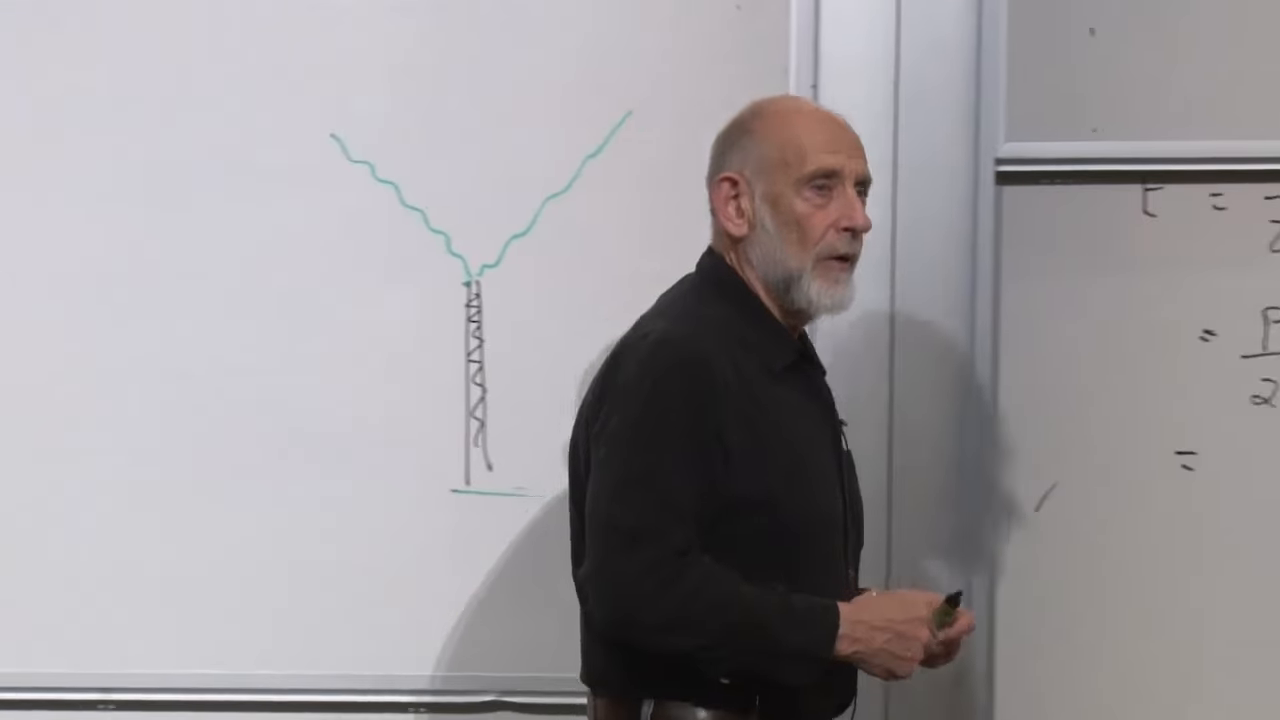
\includegraphics[width=0.90\textwidth]{lecture_03_figure_23.png}
\caption{正电子素世界线终止于一个衰变事件，两条零光子世界线从该事件发出。}
\lectureframe{01:53:48}
\end{figure}

\begin{classroomqa}
\audiencequestion{是什么决定了两个光子出射所沿的轴？}
\lecturerresponse{对于非极化态，存在量子角分布，而单次衰变会从该分布中随机选择一个方向。一旦一个方向成为现实，动量守恒就固定两个光子背对背；它并不预先选定该轴。\lecturetimestamp{01:53:55}}
\end{classroomqa}

\section{自由运动方程说明了什么}

不变量作用量并非通过猜测力律而选定。它被选为最简单的局部洛伦兹标量，并在低速下重现牛顿自由粒子拉格朗日量。对其变分得到
\begin{equation}
\frac{d}{dt}\left(\frac{\partial L}{\partial\dot x^i}\right)=0,
\end{equation}
因此
\begin{equation}
\frac{dp_i}{dt}=0.
\end{equation}
对于固定的非零质量，这等价于四维速度恒定：
\begin{equation}
\frac{du^\mu}{d\tau}=0.
\end{equation}
因此世界线在时空中是一条直线。这一单一的几何陈述同时包含均匀速率和不变的空间方向。

\begin{classroomqa}
\audiencequestion{是否存在一种更自下而上的理由来支持相对论作用量，类似于选择经典作用量以重现牛顿方程？}
\lecturerresponse{对于自由粒子，洛伦兹不变性、沿世界线的局域性以及牛顿低速极限将最简单的作用量确定到整体常数。其欧拉--拉格朗日方程随后给出动量恒定，正是无外力牛顿结果。相互作用提供进一步检验；稍后带电粒子将与电场和磁场耦合。\lecturetimestamp{01:54:27}}
\end{classroomqa}

\section{两个独立的经典极限}

非相对论极限与量子力学的经典极限是不同的操作。相对论修正由比值\(v/c\)控制。量子效应由相对于\(\hbar\)的作用量尺度控制，并结合质量、系统大小以及外力变化有多平滑等性质。

\begin{classroomqa}
\audiencequestion{恢复牛顿力学的低速极限，是否就是量子力学变为经典的同一极限？}
\lecturerresponse{不是。相对论极限涉及\(v/c\)；量子到经典的极限涉及\(\hbar\)相对于特征作用量，并且通常在大质量或力平滑变化时变得有效。一个系统可以是量子但非相对论的、相对论但本质经典的、两者兼具，或两者皆非。\lecturetimestamp{01:57:32}}
\end{classroomqa}

\begin{classroomqa}
\audiencequestion{狭义相对论与量子力学之间是否存在不相容性？}
\lecturerresponse{不存在。相对论量子理论是自洽的，并导向量子场论。著名且尚未解决的张力涉及将引力纳入量子力学，而不是将狭义相对论与量子原理结合起来。引力尚未进入当前自由粒子的讨论。\lecturetimestamp{01:59:01}}
\end{classroomqa}

目前，无外力结果已经完整：有质量粒子沿一条类时直线世界线运动，其不变质量固定其四维动量的范数，而能量和动量是同一个守恒客体的四个分量。引入电荷和电磁场将是超越这一自由运动的下一步。
